\documentclass[12pt]{article}

% for footnotes
\makeatletter
\newcommand\footnoteref[1]{\protected@xdef\@thefnmark{\ref{#1}}\@footnotemark}
\makeatother

\usepackage{common}
\usepackage{macros}
\usepackage{nameref}
\usepackage{pdflscape}
\newcommand{\sts}{Seq2Seq}
\newcommand{\embed}{\mathsf{embed}}
\title{HW3: Neural Machine Translation}
\author{Jiafeng Chen \and Yufeng Ling \and
Francisco Rivera}

\begin{document}

\maketitle

\section{Introduction}
In this writeup we consider neural machine translation---given a source sentence in one language, can we generate a target sentence in another? We work with the prevailing encoder-decoder architecture, where one neural network, the \emph{encoder}, maps the source sentence into a numerical tensor---which is supposed to be a latent representation of the source sentence. Another network, the \emph{decoder}, is a language model that takes the encoded sentence as an input, and generates a sentence in the target language. 

\section{Problem Description}
In this writeup, we consider the problem of machine translation. Let 
\begin{equation}
	\bm x_i = [x_{i1},\ldots,x_{iS}]
\end{equation}
be a source sentence, where each word belongs to some source vocabulary, $x_{it} \in \mathcal V_s$. Let 
\begin{equation}
	\bm y_i = [y_{i1},\ldots,y_{iT}]
\end{equation}
be a target sentence, with each target word belonging to some target vocabulary, $y_{it} \in \mathcal V_t$. Our goal is to learn $p(\bm y_i \mid \bm x_i)$. We often treat the prediction like a language model---i.e. we consider the sequential conditional distributions $p(y_{it} \mid y_{i1},\ldots,y_{i,t-1}, \bm x_i)$.


\section{Model and Algorithms}

\subsection{Sequence-to-Sequence (\sts)}
\label{sub:seq2seq}
In \sts{} \TODO{citation}, we have a encoder-decoder network architecture. The \emph{encoder}, in the vanilla \sts{} implementation, is an LSTM network that takes an embedding of the source sentence $\embed(\bm x_{i1}),\ldots,\embed(\bm x_{iS})$ and outputs a list of hidden states $\bm h_{i1},\ldots, \bm h_{iS}$ and cell state $\bm c_{iS}$.

In \sts{}, the decoder is another LSTM which is initialized with $\bm h_{iS}$ and $\bm c_{iS}$. At training time, the decoder LSTM takes embeddings of the ground truth target $\embed(y_{it})$ and output probability predictions for $y_{i,t+1}$. These predictions are penalized with the usual cross entropy loss at training time. At prediction time, the decoder LSTM gets passed the start-of-sentence token \texttt{<s>} and outputs predictions for the first word. We then iteratively pass in its top predictions to obtain predictions for future words. For instance, a greedy algorithm to generate a sentence would be taking the top prediction every time and pass the predicted sentence so far into the decoder to obtain the next word---stopping when the end-of-sentence token \texttt{</s>} is the top prediction.\footnote{This corresponds to beam search with beam size 1.}  

\subsection{Attention}
\label{sub:attn}
The attention model builds upon the Sequence-to-Sequence model described in section (\ref{sub:seq2seq}). Instead of only using the end state of the encoded input as input, we take advantage of a bi-directional RNN and generate target sentence by taking in a weighted input of all the states of the encoder. The intuition is that when we are translating a sentence, the adjacent words of the current word also help inform how we should translate the current word. Such weighted average is aptly named ``context''. To formalize this, we let the sequential conditional distribution be given by
\begin{equation}
	p(y_{it} \mid y_{i1}, \dots, y_{i,t-1}, \bm x_i) = g(y_{i,t-1}, s_t, c_t)
\end{equation}
where $s_t$ is the hidden state from BiRNN at time $t$ defined by
\begin{equation}
	s_t = f(s_{t-1}, y_{i,t-1}, c_t).
\end{equation}
As mentioned above, the context vector $c_t$ is a weighted average given by
\begin{equation}
	c_t = \sum_{j=1}^{T_x} \alpha_{tj} h_j
\end{equation}
where the annotations $\{h_j\}$ are the concatenated hidden states of the BiRNN and $\{\alpha_{tj}\}$ are the weights, which usually center around the current state $t$. The weights 
\begin{equation}
	\alpha_{tj} = \frac{\exp(e_{tj})}{\sum_{k=1}^{T_x} \exp(e_tk)}
\end{equation}
are generated by softmaxing over
\begin{equation}
	e_{tk} = a(s_{t-1}, h_k)
\end{equation}
for some function $a$. In our model, we take $a$ to be the dot product between the two arguments.

\begin{figure}
	\centering
	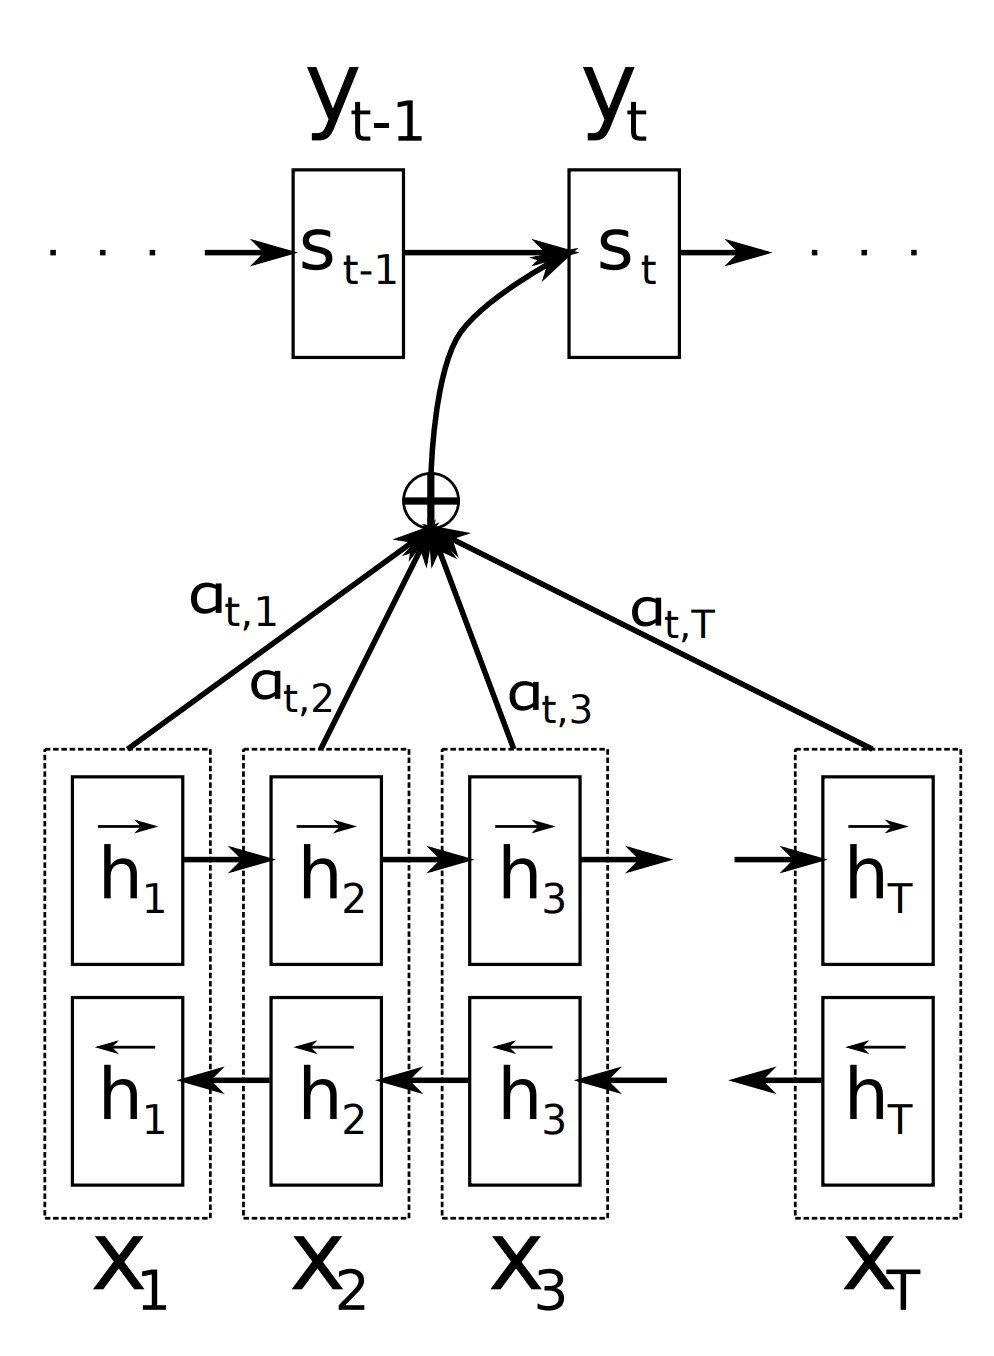
\includegraphics[width=0.4\linewidth]{figs/attn_diagram}
	\caption{Attention Diagram}
	\label{attn_diagram}
\end{figure}


\subsection{Beam Search}
\label{sub:beam}
After we have trained a model, since the outputs are conditional probabilities over the entire vocabulary, we need to have an algorithm that generates the top $k$ most likely sentences. One can use the greedy algorithm by selecting the local MLE conditional on the previously selected words. However, this can easily run into problems like stucking at a local optimum.

Beam search is proposed based on this idea. Instead of selecting the MLE, we select the top $B$ words with the largest conditional probabilities. The parameter $B$ is known as the ``beam width''. At every step, we choose the top $B$ words with the highest joint probability conditional on the $B$ previously generated sentenses $\{\bm y_{i, 1:t-1}^{(b)}\}_{b=1}^B$. That is
\begin{align}
	&\arg \max_{y_{it}, b} p(y_{it}, y_{i,t-1}^{(b)}, \dots, y_{i1}^{(b)}, \bm x_i)\nonumber\\
	=& \arg \max_{y_{it}, b} p(y_{it} \mid y_{i,t-1}^{(b)}, \dots, y_{i1}^{(b)}, \bm x_i) p(y_{i,t-1}^{(b)}, \dots, y_{i1}^{(b)}, \bm x_i).
\end{align}
And in the last step we choose the top $k$ to report as results based on given the variance parameter $k$.

\section{Experiments}


\bibliographystyle{apalike}
\bibliography{writeup}

\appendix
\section{Model implementation}


\end{document}
